
\documentclass{article}
\usepackage[final]{neurips_2019}

\makeatletter
\renewcommand{\@noticestring}{Deep Learning, Sommer 2019, Universiteit van Amsterdam}
\makeatother

\usepackage{comment}
\usepackage{amsmath}
\usepackage{amssymb}
\usepackage{multirow}
\usepackage{verbatim}

\usepackage{hyperref}
\usepackage{algorithm}
\usepackage{algpseudocode}
\usepackage{nicefrac}
\usepackage{graphicx}
\usepackage{caption}
\usepackage{subcaption}
\usepackage{dsfont}
\usepackage{bm}
\usepackage[utf8]{inputenc}
\usepackage[T1]{fontenc}
\usepackage{url}
\usepackage{booktabs}
\usepackage{microtype}
\usepackage{tabularx}
\usepackage{extarrows}

% Matrices
\newcommand\bM[1]{\ensuremath{\begin{bmatrix}#1\end{bmatrix}}}
\newcommand\vM[1]{\ensuremath{\begin{vmatrix}#1\end{vmatrix}}}
\newcommand\BM[1]{\ensuremath{\begin{Bmatrix}#1\end{Bmatrix}}}

% operators and fractions
\newcommand\·{\ensuremath{\cdot}}
\newcommand\…{\ensuremath{\dots}}
\newcommand\p{\ensuremath{\partial}}
\renewcommand\t{\ensuremath{\times}}
\DeclareMathOperator*{\argmax}{arg\,max}
\DeclareMathOperator*{\argmin}{arg\,min}
\DeclareMathOperator{\adj}{Adj}
\DeclareMathOperator{\Tr}{Tr}
\DeclareMathOperator{\Dir}{Dir}
\DeclareMathOperator{\sgn}{sgn}
\DeclareMathOperator{\soft}{softmax}
\DeclareMathOperator{\diag}{diag}

% unicode to latex
\newcommand{\⇔}{\ensuremath{\iff}}
\newcommand{\⇐}{\ensuremath{\impliedby}}
\newcommand{\⇒}{\ensuremath{\implies}}

\newcommand\f[2]{\ensuremath{\frac{#1}{#2}}}
\newcommand\nf[2]{\ensuremath{\nicefrac{#1}{#2}}}
\newcommand\pf[2]{\ensuremath{\frac{\partial {#1}}{\partial {#2}}}}

% Typesetting and symbols
\newcommand*{\B}[1]{\ifmmode\bm{#1}\else\textbf{#1}\fi}
\newcommand*{\I}[1]{\ifmmode\mathit{#1}\else\textit{#1}\fi}
\newcommand\1{\ensuremath{\mathds{1}}}
\newcommand\E{\ensuremath{\mathds{E}}}
\newcommand\ℝ{\ensuremath{\mathds{R}}}
\newcommand\N{\ensuremath{\mathcal{N}}}


\renewcommand{\thesubsubsection}{\thesubsection.\alph{subsubsection})}

\title{Assignment 1. MLPs, CNNs and Backpropagation}
\author{%
  Maurice Frank\\
  11650656\\
  \href{mailto:maurice.frank@posteo.de}{maurice.frank@posteo.de} \\
  Code: \href{https://github.com/morris-frank/uvadlc_practicals_2019/tree/master/assignment_1/code}{github}
}

\begin{document}
\maketitle
\section{MLP backpropagation}
\subsection{Analytical derivation of gradients}
\subsubsection{}
\begin{align*}
  \tag{$\pf{\B{x}^{(N)}}{L}$}
  \pf{L}{x_i^{(N)}}
  &= -\pf{}{x_i^{(N)}}\sum_i t_i \log x_i^{(N)}\\
  &= -t_i\·\f{1}{x_i^{(N)}}\\
  &\⇔\\
  \pf{L}{\B{x}^{(N)}}
  &= -[\dotsb \f{t_i}{x_i^{(N)}}\dotsb]\\
  &= \B{t}\oslash\B{x}^{(N)}\\
  &\in\ℝ^{d_N}
\end{align*}

\begin{align*}
  \tag{$\pf{\B{x}^{(N)}}{\tilde{\B{x}}^{(N)}}$}
  \pf{x_i^{(N)}}{\tilde{x_j}^{(N)}}
  &= \pf{}{\tilde{x}_j^{(N)}}\f{\exp{\tilde{x}_i^{(N)}}}{\sum_k \exp{\tilde{\B{x}}_k^{(N)}}}\\
  &= \f{\left(\pf{}{\tilde{x}^{(N)}_j}\exp{\tilde{x}^{(N)}_i}\right)\·\sum_k\exp{\tilde{x}^{(N)}_k} - \exp{\tilde{x}^{(N)}_i}\·\pf{}{\tilde{x}^{(N)}_j}\sum_k\exp{\tilde{x}^{(N)}_k}}{\left(\sum_k\exp{\tilde{x}^{(N)}_k}\right)^2}\\
  &= \f{\delta_{ij}\exp{\tilde{x}^{(N)}_j}}{\sum_k\exp{\tilde{x}^{(N)}_k}} - \f{\exp{\tilde{x}^{(N)}_i}\·\exp{\tilde{x}^{(N)}_j}}{\left(\sum_k\exp{\tilde{x}^{(N)}_k}\right)^2}\\
  &= \soft(\tilde{x}^{(N)}_j)\·(\delta_{ij} - \soft(\tilde{x}^{(N)}_i))\\
  &\Rightarrow\\
  \pf{\B{x}^{(N)}}{\tilde{\B{x}}^{(N)}} &= \bM{& \vdots &\\\hdots & \soft(\tilde{x}^{(N)}_j)\·(\delta_{ij} - \soft(\tilde{x}^{(N)}_i)) & \hdots\\ & \vdots &}\\
  &= \diag(\soft(\tilde{\B{x}}^{(N)})) -\soft(\tilde{\B{x}}^{(N)})\otimes \soft(\tilde{\B{x}}^{(N)})
  &\in\ℝ^{d_N\t d_N}
\end{align*}

\begin{align*}
  \tag{$\pf{\B{x}^{(l<N)}}{\tilde{\B{x}}^{(l<N)}}$}
  \pf{\B{x}^{(l<N)}}{\tilde{\B{x}}^{(l<N)}}
  &= \pf{}{\tilde{\B{x}}^{(l<N)}}\max(0,\tilde{\B{x}}^{(l<N)})\\
  &= \diag(\B{x}^{(l<N)}\oslash\tilde{\B{x}}^{(l<N)})\\
  &\in\ℝ^{d_l\t d_l}
\end{align*}

\begin{align*}
  \tag{$\pf{\tilde{\B{x}}^{(l)}}{\B{x}^{(l-1)}}$}
  \pf{\tilde{\B{x}}^{(l)}}{\B{x}^{(l-1)}}
  &= \pf{}{\B{x}^{(l-1)}} \B{W}^{(l)}\B{x}^{(l-1)} + \B{b}^{(l)}\\
  &=\B{W}^{(l)}\\
  &\in\ℝ^{d_l\t d_{l-1}}
\end{align*}

\begin{align*}
  \tag{$\pf{\tilde{\B{x}}^{(l)}}{\B{W}^{(l)}}$}
  \pf{\tilde{\B{x}}^{(l)}}{\B{W}^{(l)}}
  &= \pf{}{\B{W}^{(l)}}\B{W}^{(l)}\B{x}^{(l-1)}\\
  &= \bM{\vdots\\\pf{\tilde{\B{x}}^{(l)}_i}{\B{W}^{(l)}}\\\vdots}\\
  &\in\ℝ^{d_l\t (d_l\t d_{l-1})}\\
  &\text{with}\\
  \pf{\tilde{\B{x}}^{(l)}_i}{\B{W}^{(l)}}
  &= \bM{\vdots\\{\B{x}^{(l-1)}}^T\\\vdots}\\
  &\in\ℝ^{d_l\t d_{l-1}}
\end{align*}

\begin{align*}
  \tag{$\pf{\tilde{\B{x}}^{(l)}}{\B{b}^(l)}$}
  \pf{\tilde{\B{x}}^{(l)}}{\B{b}^{(l)}}
  &= \pf{}{\B{b}^{(l)}}\B{b}^{(l)}\\
  &= \1^{d_l\t d_l}\\
  &\in\ℝ^{d_l\t d_l}
\end{align*}
\footnote{Note the use of $\oslash$ for element-wise division, the use of $\delta$ for the Kronecker-Delta and the use of $\otimes$ for the Outer Product.}

\subsubsection{}
\begin{align*}
  \tag{$\pf{L}{\tilde{\B{x}}^{(N)}}$}
  \pf{L}{\tilde{\B{x}}^{(N)}}
  &= \pf{L}{\B{x}^{(N)}}\pf{\B{x}^{(N)}}{\tilde{\B{x}}^{(N)}}\\
  &= \pf{L}{\B{x}^{(N)}}\·\diag(\soft(\tilde{\B{x}}^{(N)})) -\soft(\tilde{\B{x}}^{(N)})\otimes \soft(\tilde{\B{x}}^{(N)})
\end{align*}

\begin{align*}
  \tag{$\pf{L}{\tilde{\B{x}}^{(l<N)}}$}
  \pf{L}{\tilde{\B{x}}^{(l<N)}}
  &= \pf{L}{\tilde{\B{x}}^{(l)}}\pf{\B{x}^{(l)}}{\tilde{\B{x}}^{(l)}}\\
  &= \pf{L}{\tilde{\B{x}}^{(l)}}\·\diag(\B{x}^{(l)}\oslash\tilde{\B{x}}^{(l)})\\
  &= \bM{\ddots & &\\ & \pf{L}{\tilde{\B{x}}^{(l)}}\·\f{x^{(l)}_i}{\tilde{x}^{(l)}_i} &\\ & &\ddots}
\end{align*}

\begin{align*}
  \tag{$\pf{L}{\B{x}^{(l<N)}}$}
  \pf{L}{\B{x}^{(l<N)}}
  &= \pf{L}{\tilde{\B{x}}^{(l+1)}}\pf{\tilde{\B{x}}^{(l+1)}}{\B{x}^{(l)}}\\
  &= \pf{L}{\tilde{\B{x}}^{(l+1)}}\·\B{W}^{(l+1)}\\
\end{align*}

\begin{align*}
  \tag{$\pf{L}{\B{W}^{(l)}}$}
  \pf{L}{\B{W}^{(l)}}
  &= \pf{L}{\tilde{\B{x}}^{(l)}} \pf{\tilde{\B{x}}^{(l)}}{\B{W}^{(l)}}\\
  &= \pf{L}{\tilde{\B{x}}^{(l)}} \bM{\vdots\\\pf{\tilde{\B{x}}^{(l)}_i}{\B{W}^{(l)}}\\\vdots}
\end{align*}

\begin{align*}
  \tag{$\pf{L}{\B{b}^{(l)}}$}
  \pf{L}{\B{b}^{(l)}}
  &= \pf{L}{\tilde{\B{x}}^{(l)}}\pf{\tilde{\B{x}}^{(l)}}{\B{b}^{(l)}}\\
  &= \pf{L}{\tilde{\B{x}}^{(l)}}\1^{d_l\t d_l}\\
  &= \pf{L}{\tilde{\B{x}}^{(l)}}
\end{align*}

\subsubsection{}
If we use a batchsize $B>1$ we have to perform the same derivations as described above but over a new batch dimension.
Meaning all matrices become tensor with the new first axis being of size $B$.
As the batch items do not interfer with each other the results will be equivalent to doing the not batched dervivatives for each item alone.
For the actual updates of the weights we gonna have a sum which can be build into the matrix computation.

\subsection{NumPy MLP}
The performance of the NumPy implementation of the MLP under differnt hyperparameter settings are show in Tabel~\ref{tab:numpy}.
The loss and accuracy curves of the best model are shown in Figure~\ref{fig:numpy}.
Source code is in files \texttt{mlp\_numpy.py}, \texttt{train\_mlp\_numpy.py} and \texttt{modules.py}.

\begin{table}
  \centering
  \begin{tabular}{ccccc}
    Layers & LR & Batch size & Test Accuracy & Test Loss\\\toprule
    100 & 2e-3 & 200 & 46.86 & 1.51\\
    10 & 2e-3 & 200 & 39.38 & 1.68\\
    200 & 1e-3 & 200 & \textbf{50.37} & \textbf{1.42}\\
    80,50 & 1e-5 & 200 & 11.17 & 2.30\\
  \end{tabular}
  \caption{Results for the NumPy MLP under different parameter settings. Layers shows the sorted list of number of neurons for the hidden layers. LR is learning rate. Reported are the highest accuracy and lowest loss on the test set during training.}
  \label{tab:numpy}
\end{table}

\begin{figure}
  \begin{tabularx}{\linewidth}{XX}
    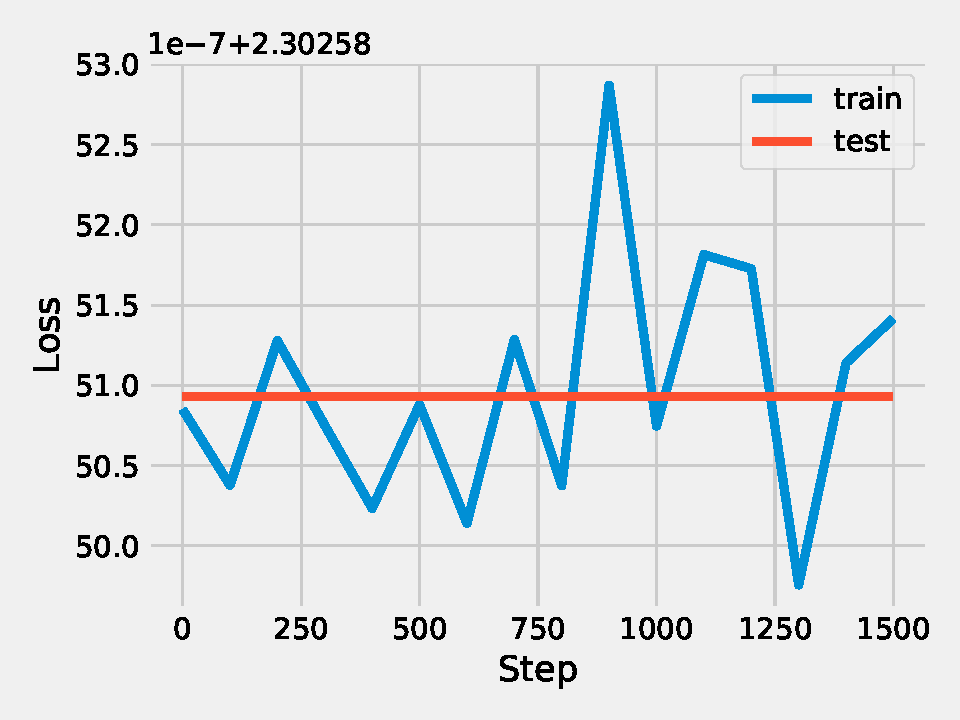
\includegraphics[width=\linewidth]{assignment_1/code/np_loss.pdf} &
    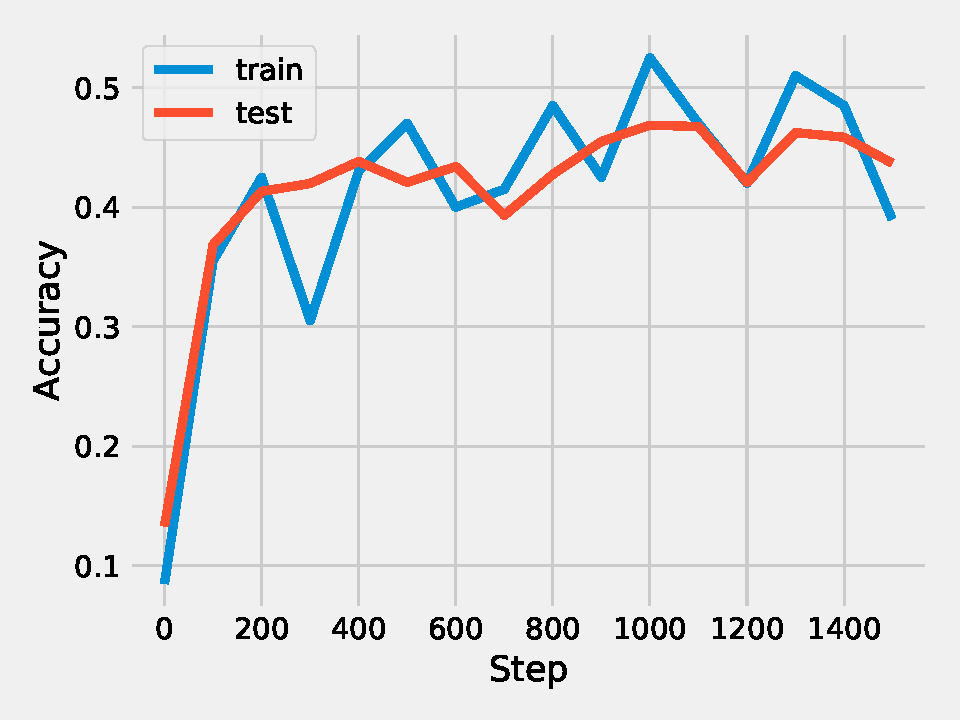
\includegraphics[width=\linewidth]{assignment_1/code/np_accuracy.pdf}
  \end{tabularx}
  \caption{\textbf{Left} the loss and \textbf{right} the accuracy during training of the NumPy MLP implementation using the default hyperparameters.}
  \label{fig:numpy}
\end{figure}

\section{PyTorch MLP}
Source code is in files \texttt{mlp\_pytorch.py} and \texttt{train\_mlp\_pytorch.py}.
The performance of the PyTorch MLP model under diffent settings are shown in Table~\ref{tab:pytorch_mlp}.
The loss and accuracy curves during training of the best performing model are shown in Figure~\ref{fig:pytorch_mlp}.
We experiment with different hyperparameter settings. We change the number of hidden neurons and the number of hidden layers.
We set different learning rates.
We use SGD and Adam.
SGD is stochastic Gradient descent with variable learning rate but we fix momentum to zero.
Alternatively we use the Adam optimizer and add regularization in the form of weight decay with a factor of $1E-2$.
The best result is achieved using Adam and three layers of decreasing size.
Generally Adam more robustly optimizes under differnt settings.
As these results  are not averages over multiple runs we see a lot of variability.
For example the single layer network with only ten nodes achieves higher accuracy than using three-hundred nodes with SGD.

\begin{table}
  \centering
  \begin{tabular}{ccccc}
    Layers & Optimizer & LR & Test Accuracy & Test Loss\\\toprule
    100         & SGD  & 2e-3 & 45.58 & 1.61\\
    10          & SGD  & 2e-3 & 39.52 & 1.70\\
    200         & SGD  & 1e-3 & 49.11 & 1.52\\
    80,50       & SGD  & 1e-5 & 31.08 & 2.26\\
    500,300     & SGD  & 1e-3 & 48.72 & 1.58 \\
    300         & SGD  & 1e-5 & 33.27 & 4.25\\
    300         & Adam & 1e-3 & 48.46 & 1.63\\
    500,300     & Adam & 1e-3 & 47.66 & 1.49\\
    600,300,100 & Adam & 1e-4 & \textbf{53.55} & \textbf{1.43}\\
  \end{tabular}
  \caption{Results of the PyTorch MLP using differnt settings for the hyperparameters. SGD is stochastic gradient descent withtout momentum.}
  \label{tab:pytorch_mlp}
\end{table}

\begin{figure}
  \begin{tabularx}{\linewidth}{XX}
    \includegraphics[width=\linewidth]{assignment_1/code/torch_loss_save.pdf} &
    \includegraphics[width=\linewidth]{assignment_1/code/torch_accuracy_save.pdf}
  \end{tabularx}
  \caption{\textbf{Left} the loss and \textbf{right} the accuracy during training of the best performing PyTorch MLP implementation. (Single layer 200 neurons)}
  \label{fig:pytorch_mlp}
\end{figure}

\section{Batch normalization}
\subsection{Autograd}
See the implementation in \texttt{custom\_batchnorm.py}: \texttt{CustomBatchNormAutograd}.

\subsection{Manual gradient}
\subsubsection{}
\begin{align*}
  \tag{$\pf{L}{\gamma}$}
  \pf{L}{\gamma}
  &= \pf{L}{y} \pf{y}{\gamma}\\
  &= \bM{\vdots\\ \sum_s\sum_i \pf{L}{y_i^s} \pf{y_i^s}{\gamma_j}\\\vdots}\\
  &= \bM{\vdots\\ \sum_s\pf{L}{y_j^s} \hat{x}_j^s\\\vdots}\\
  &= \sum_s \pf{L}{y^s}\odot\hat{x}^s
\end{align*}
\footnote{Note the use of $\odot$ for element-wise multiplication.}

\begin{align*}
  \tag{$\pf{L}{\beta}$}
  \pf{L}{\beta}
  &= \pf{L}{y} \pf{y}{\beta}\\
  &= \bM{\vdots\\ \sum_s\sum_i \pf{L}{y_i^s} \pf{y_i^s}{\beta_j}\\ \vdots}\\
  &= \bM{\vdots\\ \sum_s\pf{L}{y_j^s} \\\vdots}\\
  &= \sum_s\pf{L}{y^s}
\end{align*}

\begin{align*}
  \tag{\pf{L}{x}}
  \pf{L}{x} &= \pf{L}{(x-\mu)} + \pf{L}{\mu}\pf{\mu}{x}\\
  &\text{with}\\
  \pf{\mu}{x} &= \f{1}{B}\1^{B\t B}\\
  \pf{L}{\mu} &= -\sum_s\left(\pf{L}{(x-\mu)}\right)_s\\
  &\⇒\\
  \pf{L}{x} &= \pf{L}{(x-\mu)} -\sum_s\left(\pf{L}{(x-\mu)}\right)_s\·\f{1}{B}\1^{B\t B}
\end{align*}
so missing is $\pf{L}{(x-\mu)}$: (We set $\hat{\sigma} = \sqrt{\sigma^2 + \epsilon}$ for simplicity.)

\begin{align*}
  \pf{L}{(x-\mu)} &= \pf{L}{y}\pf{y}{\hat{x}}\pf{\hat{x}}{(x-\mu)} + \pf{L}{y}\pf{y}{\hat{x}}\pf{\hat{x}}{\nf{1}{\hat{\sigma}}}\pf{\nf{1}{\hat{\sigma}}}{\hat{\sigma}}\pf{\hat{\sigma}}{\sigma}\pf{\sigma}{(x-\mu)}\\
  &\text{with}\\
  \pf{y}{\hat{x}} &= \gamma\\
  \pf{\hat{x}}{(x-\mu)} &= \f{1}{\hat{\sigma}}\\
  &\text{and with}\\
  \pf{L}{\nf{1}{\hat{\sigma}}}
  &= \pf{L}{y}\pf{y}{\hat{x}}\pf{\hat{x}}{\nf{1}{\hat{\sigma}}}\\
  &= \sum_s \left(\pf{L}{\hat{x}}\right)_s\·(x_s-\mu_s)\\
  \pf{\nf{1}{\hat{\sigma}}}{\hat{\sigma}} &= -\f{1}{\hat{\sigma}^2}\\
  \pf{\hat{\sigma}}{\sigma} &= \f{1}{2\·\sqrt{\sigma+\epsilon}}\\
  \pf{\sigma}{(x-\mu)} &= 2\·(x-\mu)\·\f{1}{B}\1^{B\t B}\\
\end{align*}

\subsubsection{}
See implementation of the manual backward pass in \texttt{custom\_batchnorm.py}: \texttt{CustomBatchNormManualFunction}.
We use the functions context to save the five tensors $x-\mu$, $\sigma^2$, $\f{1}{\sqrt{\sigma^2 +\epsilon}}$, $\f{x-\mu}{\sqrt{\sigma^2 +\epsilon}}$ and $\gamma$.
In that we make a conscious decisions to trade time performance for more memory usage.

\subsubsection{}
See the implementation in \texttt{custom\_batchnorm.py}: \texttt{CustomBatchNormManualModule}.

\section{PyTorch CNN}
See the implementation in \texttt{convnet\_pytorch.py} and  \texttt{train\_convnet\_pytorch.py}.
Curves for loss and accuracy during training are shown in Figure~\ref{fig:pytorch_conv}.
Using the default parameters and  the Adam optimizer we reach a maximum of 77.08\% accuracy on the test set.

\begin{figure}
  \begin{tabularx}{\linewidth}{XX}
    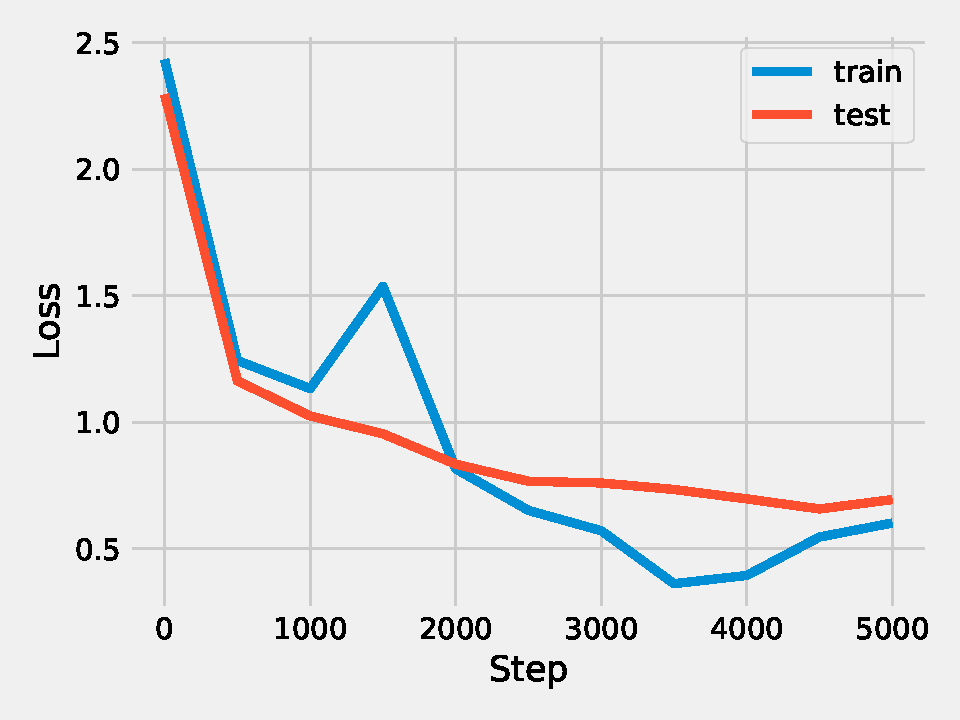
\includegraphics[width=\linewidth]{assignment_1/code/conv_loss.pdf} &
    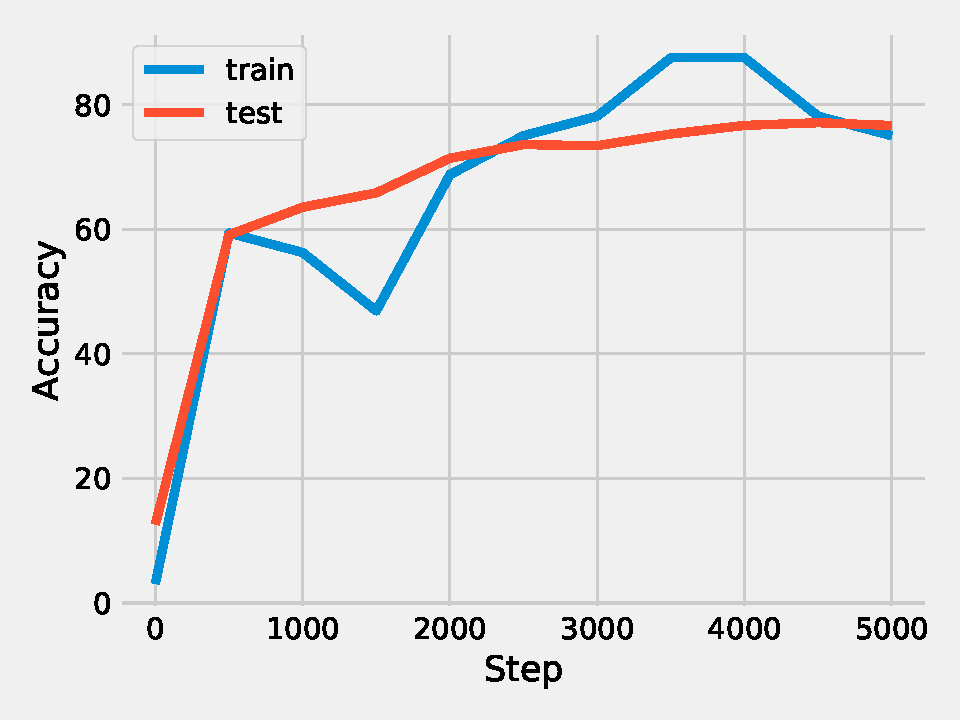
\includegraphics[width=\linewidth]{assignment_1/code/conv_accuracy.pdf}
  \end{tabularx}
  \caption{\textbf{Left} the loss and \textbf{right} the accuracy during training of the PyTorch CNN implementation.}
  \label{fig:pytorch_conv}
\end{figure}

\end{document}
